%===============================================================================
%     File: ch_machine_learning.tex
%    Author: Juan de Monasterio
%    Created: 08 Feb 2017
%  Description: Chapter : Machine Learning
%===============================================================================
\chapter{Machine Learning}
\label{ch:machineLearning}

\section{Preamble}\label{section-preamble}
Most of the discussions in this chapter are based on information extracted from two distinguished textbooks: \textcite{bishop-patternRecognition} and \textcite{hastie-elemstatslearn}. Some fundamental concepts and material were also used from\label{scikit-learn}. While other texts were also used, it is not necessary that we point them out here as they have been correctly cited. Where not specified, the reader can assume that the proof is based from said texts.


\section{ Supervised classification problems}\label{section-supervised-learning}


Machine Learning is divided into two main categories: Supervised and Unsupervised Learning. Let $Y \in \mathbb{R}^n$ be the outputs of the model and $X \in \mathbb{R}^{n \times p}$ be the inputs: supervised learning algorithms produce outputs from input data i.e.\ for each instance $n$, the computer has access to examples of outputs and tries to reproduce them based on information contained in $X$. In this context, the algorithm is generally referred to as a \textit{learner}.

The second class of problems is where the output $Y$ is missing altogether from the data. In this scenario the most common objectives are clustering samples, density estimation and data compression. Linear regression and K-means clustering are examples of algorithms in each of these categories respectively.


In supervised learning tasks can be sub-categorized by the nature of the problem. When the type of the output variable $Y$ takes a (generally \textit{small}) discrete set of values, then it is said that it is a supervised \textit{classification} problem. On the other hand, when the output takes continuous (or dense in an open set of $\mathbb{R}$) range of \textit{quantitative} values, the problem is said to be of supervised \textit{regression}. Note that regression problems can be encoded into classification problems by grouping the output values into categories by taking ranges of output values.

Suppose our aim is to predict $y$ given a new sample $x$. In supervised regression problems, $y$ will comprise a continuous variable. On the other hand for classification problems $y$ will represent a label for a certain class. For the case of $K$ classes, $y$ most commonly takes values in the ranges $0$ through $K-1$ or $1$ through $K$. In both cases, the joint probability distribution $p(X, Y)$, called the \textit{true} distribution, gives all the information we need on these two variables. But the values of this probability is most often unknown. The idea is to then user estimations and inference on the most likely values for new samples and take decisions with the information at hand. These decisions will be based on the most probabilistic characterization of the data we have. In this work we will focus on the classification aspect of machine learning.

In these type of problems the theoretical and the computational aspects are both of interest. The algorithms used need to consider the technical requirements of the software and hardware at hand, as well as the time or resource constraints imposed by the problem setting. As such, they are expected to be executed in a reasonable amount of time, imposed by the task specification, and limited by the computing power available.\footnote{Here the word \textit{reasonable} is used in a broad sense. It will depend entirely on time constraints, computational capacity, usage and other aspects of each learning application.} There can be problems which require that the algorithm output predictions in \textit{real-time}, to the resolution of milliseconds. Picture a system where a credit-card transaction needs to be approved or labeled as a fraud. Here the system needs to respond in short time if the transaction is fraudulent.

Other use cases might require the system to process a big volume of data at once, not a single event, but a batch of these and output this answer. The system in use needs to be prepared to run \textit{lean} with a big inflow of data, without overloading the hardware capacity. These examples show that for a given problem, multiple algorithms are available to use but while all of them are theoretically doing the same task, we must also consider the practical advantages of these. Computational efficiency and \textit{scalability} are relevant when working with these problems. Even though we won't delve into these aspects in this work, it has an important consideration in the application of Machine Learning solutions.


In its essence, a machine learning method is a probabilistic model built from data so it is very similar to a statistical model. However, it differs specially in that its focus is generally on the models' predictive abilities more than in the model's parameters estimates~\textcite{breiman-statisticalmodeling} The algorithms will be built and used for a given phenomena, to try and replicate it as best as possible without really identifying the true nature of the mechanisms behind this phenomena. As such, most applications will try to \textit{imitate} the task's behavior rather than try to identify the real system behind it.
%on this matter It also puts a great amount of weight on efficiency and computational scalability.

%At this point it is important to start noting

These subtle differences in the machine learning approach of a problem is also reflected in the terminology used by the field. We know that different disciplines often speak about the same machine learning methods in different terms and this difference is most notable with classic statistics. Where we can, we will be identifying these differences along the text. As a start, the \textit{dependent} $Y$ is called the target or label and the \textit{independent} variables, \textit{covariates} or \textit{input variables} are named \textit{features} in this case.
%Labels that are representing categorical or discrete variables are also named factors or \textit{qualitative} variables.

\section{Supervised Classification of Long-term Human Migrations}\label{long_term}

To better characterize migrations, we decided to divide our task into four problems. These are different perspectives of the issue and all of them together give us a better overview of the relationship of CDRs to long term migrations. These are solved using user information of how they communicated during $T_1$ whilst no information from $T_0$ will be used as input to the model.

We process the raw data to build our target variable which will be determined as $Y$. This will always be defined for every user $u$. We take $H_u$ to be the user's home antenna. The only differences among the problems will be in how the target variable will be defined.\footnote{In reality, certain variations of the data were considered too, were best performing features were filtered from the dataset to explore how this decreased the overall prediction ability of the algorithm.}


With these definitions, the list of problems considered in this work are defined in the following way:

\begin{problem}\label{target1}
We want to infer which users lived in the endemic region in the past:
		\begin{align*}
		Y_u =
		\begin{cases}
		&1 \ \mbox{if} \ H_u \in E_{Z0} \\
		&0 \ \mbox{if not}.
		\end{cases}
		\end{align*}
\end{problem}

With this definition and the description of the features extracted from the data in \cref{ch:descr-risk}, it is important to observe that we are using the information of a user's endemicity $E_{Z1}$ to predict $E_{Z0}$.
And it wouldn't be of much surprise to know that these two variables are indeed highly correlated with a value of 93\%. This means that, overall, the feature is a good predictor of the target variable causing algorithms to be heavily weighted towards this attribute. A simple enough algorithm would use this single feature as sole predictor.

To prevent this from happening and to try and capture the change in endemicity for a small groups of users, we decided then to hide the feature when solving \cref{target1}.

% Other features, such as the number of calls to endemic regions, are correlated to the target variable. This is an expected behavior since most people use cellphones for local calls only. Yet these correlations are not as high as with the $E_{Z1}$ variable. Also, given the assumptions used in

% However we have not excluded any other features
% are locally  an and given the assumptions used maps in \cref{}, this is a result which

\begin{problem}\label{target2}
We want to infer which users lived in $E_Z$ in the past and then migrated:
	\begin{align*}
				Y_u =
				\begin{cases}
					&1 \ \mbox{if} \ H_u \in E_{Z0} \cap { E_{Z1} }^{\complement}  \\
					&0 \ \mbox{if not}.
				\end{cases}
			\end{align*}
\end{problem}

In this task, we have not excluded any attributes from the data since this is a much difficult problem.
Recall from \cref{tab:changes} that we have at most 23 thousand users that satisfy this condition from more than a million users. This volume unbalance in the target class proves to be a much harder problem to solve than in \cref{target1} since these users become harder to find.

% This is because we could use a dumb predictor to always output the value of the bigger class. With this, the error over the small class would be dominated if not correctly taken into account.


\begin{problem}\label{target3}
Users that migrated to a different region.
\begin{align*}
			Y_u =
			\begin{cases}
				&1 \ \mbox{if} \ H_u \in (E_{Z0} \cap { E_{Z1} }^{\complement}) \cup (E_{Z1} \cap { E_{Z0} }^{\complement}) \\
				&0 \ \mbox{if not}.
			\end{cases}
		\end{align*}
\end{problem}

This task has a similar difficulty as in the previous one. Yet there are more users satisfying this condition.
The difference relies in that cross-migrations are not as important to our study as migrations directly from the endemic region.

\begin{problem}\label{target4}
Users that migrated from the endemic region, but only those which are currently not endemic.
\begin{align*}
			Y_u =
			\begin{cases}
				&1 \ \mbox{if} \ H_u \in (E_{Z0} \cap { E_{Z1} }^{\complement}) \forall u s.t. H_u \in E_{Z1}^{\complement}    \\
				&0 \ \mbox{if not}.
			\end{cases}
		\end{align*}
\end{problem}

Note that at this point we are looking at a reduced instance of our CDRs. That is, we are only considering currently non-endemic users other than the whole sample population. Still, we are taking more than a million users in this dataset.


% \begin{problem}\label{target5}
% As a \textbf{bonus} problem and for exemplary reasons, we considered tried to detect if a user has a high mobile footprint $M_u$, as defined in \cref{section:def_mobility_diameter}.

% 	\begin{align*}
% 		Y_u =
% 		\begin{cases}
% 			&1 \ \mbox{if} \ {M_u >  1000 } \\
% 			&0 \ \mbox{if not}.
% 		\end{cases}
% 	\end{align*}

% \end{problem}


We can see from what was mentioned before that not all problems can be represented by the same dataset.
The limitations on what is available as our input set $X$ attributes or samples. For example, we said that in \cref{target1} we have no limitations to use that $H_u$ at $E_{Z1}$, yet we decide to ignore this highly correlated feature. As a result, we  would be implicitly introducing the target variable as an attribute.
With this in mind, appropriate care must be taken for each case on which attributes are available for the problem being analyzed.


With \cref{target1,target2,target3,target4}, we continue onto define and illustrate techniques for supervised classification. Throughout \cref{ch:modelSelection,ch:ensembleMethods,ch:results_conclusion} we will come back to these problems by applying them with the techniques and methods we discuss.


\section{A working example of a Machine Learning setup}\label{section-example}

From now on we will be talking of the training set and the test set, noted by $\mathcal{T}$  and $\mathcal{T_s}$ as our two data sources. The test set will be a part of the whole dataset that will only used at the end of the algorithmic process. This set will not take part in building the machine learning model and will be used only to evaluate its performance. This makes sense knowing that the objective is to build a probabilistic model which has the capacity to correctly predict the class instances of new data objects, such as those from $\mathcal{T_s}$, based on having seen information of objects from $\mathcal{T}$.

As an example, let's consider a reduced training dataset built from Call Detail Records (CDRs) where samples are calls being made by users who can belong to any of the following provinces: \textit{Buenos Aires}, \textit{Cordoba} and \textit{Santa Fe}.
%\url{http://stackoverflow.com/}
%\footnote{For more information on this set, a historic review is given at \url{https://en.wikipedia.org/wiki/Iris_flower_data_set}}.
Five measurements were taken on all of the observations to account for the user's number of calls and total minute duration of calls. All data was extracted from a week of logging measurements. Below we print a short overview of this dataset:

\begin{table}[ht]
\caption{{Head of the CDR dataset. A three-row mock example.}}
\label{tab:sample_CDR}
\centering
\begin{tabular}{ l l l l l l }
\toprule
User & CallsWeekend & TimeWeekend & CallsWeekDays & TimeWeekday & Province \\
\midrule
BA343E & 15 & 89 & 8 & 24 & \textit{Santa Fe}\\
73F169 & 10 & 121 & 2 & 98 & \textit{Cordoba} \\
EA23AD & 12 & 43 & 5 & 154 & \textit{Buenos Aires} \\
\bottomrule
\end{tabular}
\end{table}

In this form a row is representing the available data acquired from each user and the columns represent the features which are the different types of measurements or information on that user. In general, most machine learning problems will be associated with a training set $\mathcal{T}$ of similar form as the one shown before. And it is common to represent data in with rows as observations or \textit{samples} and columns are measurements or \textit{features} of our samples.

Both $\mathcal{T}$ and $\mathcal{T_s}$ will take the form of a paired couple of datasets $(X,Y)$ where $X \in \mathbb{R}^{n \times p}$ and $Y \in \mathbb{R}^n $. The difference will lie in the way each set is used to computationally build a probabilistic model. In essence the former is used to algorithmically create a function which maps inputs to outputs,  whilst the latter will be used to measure how \textit{well} this mapping would behave in real situations, given a way of measuring this performance.

More specifically, the $jth$ column of $X$ or equivalently the $jth$ feature of the dataset is denoted by $X^j$. In a similar way, the $ith$ row or sample of $X$ is denoted by $X_i$ or $x$ when it is clear from context or when we are referring to a generic sample. A similar notation is used with the outputs, where $Y_i$ or $y$ will be used to denote the target of a specific sample depending on context.

In this particular example, even though the last column of the dataset in \cref{tab:sample_CDR} is not a measurement \textit{per se}, it provides information on each user's province of residence. With this we can map users to \textit{classes} which conform the partition of the set of provinces.

Hereon, there are various questions one could try to answer using this dataset. Examples of problems that a machine learning algorithm could tackle could be:

\begin{itemize}
\item Predict a user's province when given information on only the first four features.
\item Predict a user's number of calls made on weekends when given information on the last four features.
\item Give an estimate of the probability density function of user's calls duration, during weekdays.
\end{itemize}

These questions can be shaped into the form of a target variable. In this way, they become our machine learning problem.

The first two problems are examples of supervised learning task. For each, the $Y$ variables or \textit{labels} are respectively the last and first features (columns in the dataset). Even more, the first problem is a classification one since users are to be categorized according to one of the three possible provinces, whilst the second one is a regression problem for which the output could be any of a range of numerical values. The labels in classification problems are numerically encoded with a finite range of numbers where $\{0,1\}$ or $\{-1,1\}$ are usually used in the binary class problem.

Note that we are not making any assumptions on the data which we take as given. %to us in this way.
This is common in machine learning applications and because of this, algorithms tend to be designed to account for this lack of context. The type of problems and questions that could be done, then depend entirely on the data.

From the list before, the last example belongs to the unsupervised learning category where there is no need to have a label on the data. A priori, the data doesn't' give any examples of this. Here the question is on the structure of a specific column, namely the estimation of the true probability distribution of the calling time. As such, there is no output expected from new data. For the most of this work, we will be talking about supervised classification scenario.

To further illustrate this scenario, we briefly introduce some notation below. For this task, we build a standard logistic regression classifier:

Let's suppose that we want to build a predictive model to determine the origin province of a user. A classification algorithm should assign samples to provinces. Let $\{C_1,..,C_k\}$ denote the set of possible target classes. Our aim is to maximize the probability of belonging to a certain class, given the phone data:
\begin{equation}
P(C_k| X) = \frac{P(x|C_k)P(C_k)}{P(x)}
\end{equation}

In this interpretation, $P(C_k)$ is known as the prior probability of belonging to that certain class and $P(C_k|x)$ as the posterior probability, given the sample data.

Our classifiers will partition the input space into decision regions $R_k$ for which a class $C_k$ is uniquely associated to a region. It makes sense to try and \textit{minimize} the chances of assigning samples to incorrect regions. For example, take a problem with $K$ classes. Given a sample $x_i$, the probability $P$ of a correct classification,with probability density function $p$, is measured by

\begin{equation}\label{eq:goodclassification-equation}
\begin{split}
= & \sum_{k=1}^{K} P(x_i \in R_k, C_k ) \\
= & \sum_{k=1}^{K} \int_{R_k}p(x_i,C_k) dx \\
= & \sum_{k=1}^{K} \int_{R_k}p(C_k \mid x_i) p(x_i) dx
\end{split}
\end{equation}

Observe that the measure is completely characterized by the posterior probabilities. The factor $p(x)$ is common to all integrals so we only need to maximize the posteriors. And even when $p(x)$ might not be known or accurately estimated, the algorithm can only modify the decision regions $R_k$. This will have a direct effect on the probability of correctly classifying samples. Thus the goal of our algorithm will be to choose the best possible regions for the problem.

In our example, a reduced problem instance would be to determine if a user belongs to the province of \textit{Cordoba} vs the rest of the provinces. This brings us to a binary classification problem since there are two possible output classes. %us to a two class learning problem.

As a simple solution to predict the target variable, we could build a learner $f$ from a transformed linear combination of the input features. In the ideal case we would have that for every sample $y \approx f(x) = h\left(\sum_{j}\theta^j x^j\right)$\label{formula:1} where $\theta$ is unknown and generally referred to as the coefficient or parameter\footnote{In formula\cref{formula:1} we have omitted the intercept parameter, generally noted as $\theta_0$. The reason for this is that one can include this parameter implicitly if we allow for a synthetic feature $X^0$ in $X$ which is a vector with all its components equal to 1.}. Here the model is said to be \textit{linear} because it is linear in the input space $X$.

If we let our decision boundary be $ t_i = \theta \cdot x_i \ \forall \ i $,in the ideal case we will have that $\exists \theta s.t. \forall i $

\begin{equation}
t_i
\begin{cases}
&>0 \ \mbox{if} \ y_i=1 \\
&<0 \ \mbox{if} \ y_i=0.
\end{cases}
\end{equation}
%    \forall 1 \leq i \leq n = y^i $

As an example, we could take the heavy-side step function as our transformation $h(z)$ where

\begin{equation}
h(z) =
\begin{cases}
&0 \ \mbox{if} \ z<0 \\
&\frac{1}{2} \ \mbox{if} \ z=0 \\
&1 \ \mbox{if} \ z>0.
\end{cases}
\end{equation}

If the goal of the model is to maximize $P(Y_i = y_i | X_i = x) \ \forall i$
under the assumption that $\nexists\ i \ / \ t_i = 0$, the algorithm would then correctly classify all samples to their targets. Yet this situation is hardly the case. The common approach is then to rely on optimization procedures to minimize the amount of misclassification given by our algorithm. This would be analogous to maximizing the probability of a correct classification in \cref{eq:goodclassification-equation}.

\todo{fix formulas here. Some are badly written/wrong.}
For analytical convenience, a more tractable function for this task is the logistic which is an approximation of the heavy-side step function. Here

\begin{equation}\label{eq:logisticFunction}
\sigma(z) = \frac{e^{z}}{1 + e^{z}} = \frac{1}{1 + e^{-z}}
\end{equation}

where we use the relation

\begin{equation}
 \ H(z) = \lim_{k \to \infty} \left(\frac{1}{2} + \frac{1}{2}\tanh(kz) \right) = \lim_{k \to \infty} \left(\frac{1}{1+e^{-kz}} \right)
\end{equation}

The logistic function has the advantage of being smooth, well defined for all real numbers and with its image in $(0,1)$. This property lends itself to reading outputs as probabilities of targets belonging to a certain class.

 Its derivative can be put in terms of the logistic function itself, where

\begin{equation}\label{eq:derivativeLogisticFunction}
\sigma '(a) = \sigma(a)( 1 - \sigma(a) )
\end{equation}

It is also bijective, with the inverse given by the \textit{logit} function

\begin{equation}\label{eq:logitFunction}
\sigma^{-1}(z) = \log( \frac{z}{1 - z})
\end{equation}

For the scenario characterized in \cref{formula:1} we would have to finally assign each output to a specific class. A common approach for this is to categorize each output whether $\hat{y} > 0.5$\label{formula:logitThreshold}. Notice that having $h(x \cdot \theta) = 0.5$ implies that $x \cdot \theta = 0$ and thus our classifier is separating samples in feature space (the space of the inputs) with the hyper-plane defined by the parameter $\theta$. Having a higher $\hat{y}$ for a given sample implies that it is further away from the hyper-plane. The same goes for low estimated targets. If we were to read this as a probability, we can interpret that the algorithm is modeling the posterior probability $P(Y_i = y | X_i = x)$ and would correspond to having a higher confidence in the classification.

%This means that

%It also happens to be an approximating function to the


\section{Logistic Regression for Classification}\label{section-logisticRegression}

This model is named as a \textit{regression} model but is actually used for \textit{classification} and this convention has been made this way for historical reasons.


Let $\{C_1,..,C_k\}$ denote the set of possible target classes. Recall that in a classification problem we are interested in maximizing a sample's probability of belonging to a certain class, given the input data:

\begin{equation}
P(C_k| x) = \frac{P(x|C_k)P(C_k)}{P(x)}
\end{equation}

As a simple case, in the two-class problem we have that


\begin{equation}
\begin{split}
P(C_1| x) & = \frac{P(x|C_1) }{P(x|C_1)p(C_1) + P(x|C_2)p(C_2)} \\
& = \frac{1 }
{1 + \exp(- \log(  \frac{ P(x|C_1)p(C_1)}
{P(x|C_2)p(C_2)
}))
}
\end{split}
\end{equation}

Here we see the close resemblance to the logistic function which is acting on the \textit{log-odds ratio} $ \log(  \frac{ P(x|C_1)p(C_1)}{P(x|C_2)p(C_2) })$. This equivalent form of the posterior distribution of one class with regards to the log-odds one property defining the model.


%\begin{definition}{Logistic Regression}
%xGiven a choice of parameter $\theta$,
%\end{definition}

The second defining property of logistic regression is that the log-odds are modeled with a transformation on a linear combination of inputs. It also conditions the posterior probabilities must sum to one. Let $j$ be a fixed class and denote

\begin{equation}\label{logit-logOddss}
 \log\big( \frac{P(C_i|x)}{P(C_j|x)}\big) = \theta_{i0} + \theta_i^\intercal \cdot x
 \end{equation}  for $i,j \in \{1,2,\ldots,K\}, i\neq j$

With these same indices we have that

\begin{equation} P(C_i|x) = \frac{\exp(\theta_{i0} + \theta_i^\intercal x)}{1 + \exp(\theta_{j0} + \theta_j^\intercal x)}
\end{equation}

In this way the model is specified in terms of the log-odds for each class with respect to the base class $j$ and the model will be parameterized by $\theta$.

The model then sets the target as a Bernoulli random variable when conditioned on the input variables. Formally we have that,

\begin{equation}
\begin{split}
Y_i \mid X_i \ \sim & \operatorname{Bernoulli}(p_i) \\
\mathbb{E}[Y_i \mid X_i ] = & p_i
\end{split}
\end{equation}


The probability function of the target given the features $\Pr(Y_i=y\mid X_i)$ is given by
\begin{equation}\label{logit-probabilityDensity}
\Pr(Y_i=y \mid X_i = x_i) = p_i \ I(y=0) + (1-p_i) \ I(y=1) = p_i^{y} {(1-p_i)}^{(1-y)}
\end{equation}

where this depends on the class dependence of $y$.

Here the logit function is utilized to map log odds into conditional probabilities and the model outputs the predicted probabilities of the target variables belonging to a certain class.

This is why we are specifying a model where the target is a linear function of the inputs, corrected by an error term. Our model will then be characterized by:
\begin{equation}\label{logit-indicatorFunction}
Y_i = I(\theta_0 + \theta \cdot X_i + \epsilon > \frac{1}{2}) \ \forall i
\end{equation}.

where $\epsilon$ is the error of the approximation and is distributed with the standard logistic distribution. %and \dfrac{num}{den}parameter $p_i$.

If we take the conditional probability in \cref{logit-indicatorFunction}, given the features we will have that
\begin{equation}
logit(p_i)= \ln(\frac{p_i}{1-p_i}) = logit\big( \Expect[Y_i| X_i] \big) = \theta_0 + \theta \cdot X_i
\end{equation}

By an abuse of notation, we absorb $\theta_0$ into $X_i$. This can be safely done if we consider a dummy attribute $X_i^0$ which is always equal to $1$ for every sample $i$. Then from the equation above we have that

\begin{equation}
p_i = \sigma(\theta \cdot X_i) = \frac{\exp(\theta \cdot X_i) }{1 + \exp(\theta \cdot X_i)}
\end{equation}

Finally, using this $p_i$ representation and plugging it into the initial conditional probability of $Y_i$ in \cref{logit-probabilityDensity} we will have

\begin{equation}
 \Pr(Y_i=y \mid X_i = x_i) = p_i^{y} {(1-p_i)}^{(1-y)} = \frac{\exp(\theta \cdot X_i) }{1 + \exp(\theta \cdot X_i)}
 \end{equation}


Maximum likelihood is the most common method employed to fit the model. %with multinomial distributions modeling the features.
Given a parameter $\theta$, the probability of having a target vector $y$ is

\begin{equation}
P(Y =y \mid \theta ) = \prod_{i=1}^N {P(y_1 \in C_1 \mid x_i, \theta)}^{y_i} {(1 - P(y_1 \in C_1 \mid x_i, \theta) )}^{(1-y_i)}
\end{equation}

If we take into account that $P(y=1 \mid x,\theta) = 1 - P(y=0 \mid x,\theta)$ and the logistic function's derivative form \cref{eq:logitFunction}, then the estimation of $\theta$ for $N$ samples gives the following form
loss function

\begin{equation}\label{eq:logLossFunction}
l(\theta) = \sum_{i=1}^N \big(y_i \log(P(y_i \mid x_i,\theta)) + (1-y_i)\log(1 - P(y_i \mid x_i,\theta) ) \big)
\end{equation}

In Machine Learning this is called the log loss function. It is used as a metric or score function of the quality of $\theta$ in correctly assigning estimated targets $ {\hat{p_i}} = P(y_i \mid x_i,\theta)$ for the model defined by $\theta$ and the input data $X$.

\begin{definition}{Loss Function}

The loss function of a model $l: \mathbb{R}^{ p} \rightarrow  \mathbb{R} $ maps the model's parameters a quantification of a model's error when using parameter $\theta$.
\end{definition}

The loss function will define the underlying optimization procedure behind the Machine Learning problem. From this function we will output the optimum $\theta*$ as the $\argmin_{\theta} l(\theta) $. Thus we say that loss or scoring functions give us a way to find the best parameters for our model.

Note however, that the optimum parameter will be dependent on the choice of the algorithm used to construct the model. That is, we have selected the optimum $\theta$ for a Logistic Classifier with input data $X$. Other algorithms can be used for the same task, and these will have their own parameters and scores.

In our derivation, the scoring function was constructed from the assumptions proposed at the start. However, we could in fact build \textit{any} type of algorithm which given an input $x_i$ and a parametrization of the model $\theta$, outputs a value $P(y_i \mid x_i,\theta)$. And we could in fact compare the performance of that model to the one built by a Logistic Regression Classifier by using the same log loss function for both. Thus we have introduced a way of determining how to select a model from the data.

In the case of \cref{eq:logLossFunction} we have that it is a concave, monotone increasing function. The \cref{figure-logLossValues} expands on the values of this function:

\begin{figure}[h!]
\begin{center}
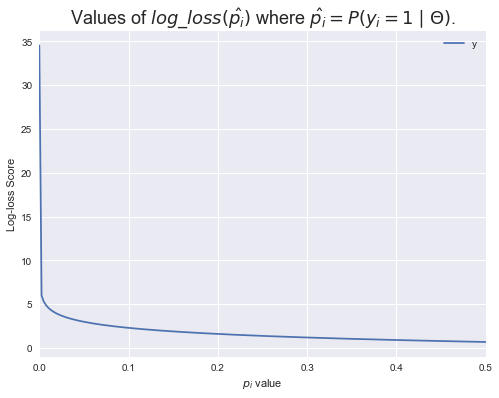
\includegraphics[width=0.7\columnwidth]{figures/logloss/figure-logLossValues.png}
\caption{ Series plot for different values of the log loss function used as an error score.}
\label{figure-logLossValues}
\end{center}
\end{figure}

As we can see, the function is much more negative for small values near zero than it is positive for large values near one. This means that it penalizes strongly on wrong predictions, for samples where the algorithm has a strong confidence that won't be of the positive class. Another advantage is that the function is concave in the parameters. This means that the optimization procedure will always, if converged, stop at a global optima.

Finally, the closed form given by the logistic regression model has the benefit that explicit forms can be given for the gradient and the Hessian of the loss function with regard to the whole dataset $X$ as a sum involving individual samples $x$.

The negative gradient can be expressed in the following way: %can thus be analytically expressed

\begin{equation}\label{eq:logitHessian1}
- \nabla l(\theta) = \sum_{i=1}^N (y_i - P(y_i \mid x_i,\theta))\cdot x_i = \textbf{X}^{\intercal}(\textbf{y}-\textbf{p})
\end{equation}

whilst the Hessian takes the following form:

\begin{equation}\label{eq:logitHessian2}
\frac{\partial^2 l(\theta)}{\partial \theta \partial \theta^\intercal} = \sum_{i=1}^N x_i \cdot x_i^\intercal P(y_i \mid x_i,\theta)(1 -P(y_i \mid x_i,\theta))
\end{equation}

From the derivations above, we can now fit $\theta$ using an optimization procedure that would take advantage of having the closed-form representations of the first and second derivatives of the loss function.


\section{Model Regularization and Hyper-parameters}\label{section-hyperParametersRegularization}


\begin{definition}{Model Regularization}

Regularization of models is the process in which restrictions and conditions are imposed on the model's function $f$ through a functional $ R(f)$. The regularization term is used in the optimization procedure through the scoring function.

\end{definition}

Regularization is used in problems which are ill-posed either because the model has very different performance in the training vs the test set's performance. In general, restrictions are added to the model in order to reduce the number of predictors used.

This \textit{shrinkage} of parameters can be forced by penalizing large values for $\theta$ either by the number of non-null components of this parameter or by measuring its distance to zero. By doing so, we hope that only the most relevant features are selected in the final model. As we will see in \cref{section-VcDimension}, a shorter model has the benefit of being more accurate in the estimation of the prediction error. In other cases, the benefit of a reduction in the number of features is that the overall variance of the predictions are reduced, only with a slight increase in error. A slightly more \textit{heuristic} argument for model parsimony is that as such, all models will approximate nature up to a certain level; and if two models have the same predictive power, the simpler model should be used.


There is a number of different functionals $R(\cdot)$ used to impose conditions on the model. The most common ones include introducing a penalty to the size of $\theta$ by measuring a given norm $\| \theta \|$. Most implementations of the algorithms use $l1$ and $l2$ norms.

Each has its advantages and the details exceed the nature of this work. As a summary, benefits are related to the robustness of the solution, convexity of the minimization function, unique minimum and model parsimony. The former case is known as \textit{ Lasso} regularization and the latter is known as \textit{ridge} or \textit{Tikhonov} regularization. Other variants include the \textit{elastic-net} penalty which is a weighted average of the previous two norms, or the $l_0$ norm, which is the number of non null components of $\theta$.


In practice, optimal solutions $\theta*$ are searched by iterative optimizations on loss functions.
For some specific algorithms though, closed-form solutions can be used, even with regularized scoring functions.
However for the former case, gradient descent is by far the most widely practiced routine.

The following example shows the logistic regression's model loss function with an $l2$ regularization term on $\theta$:

\begin{equation}\label{eq:logitRegularization}
\begin{split}
\min_{\theta} & \sum_{i=1}^N \big(y_i ( \theta \cdot x_i ) + \log(1 + e^{\theta \cdot x_i} ) \big) + \lambda { \| \theta \|_{2}}^2 \\
\min_{\theta} & \sum_{i=1}^N \big(y_i ( \theta \cdot x_i ) + \log(1 + e^{\theta \cdot x_i} ) \big) + \lambda \sum_{j=1}^P \theta_j^2
\end{split}
\end{equation}

%\min_{\theta} & \sum_{i=1}^N L(f(X_i,\theta),Y_i)  + \lambda\| \theta\|_{2}^2 \\
%\min_{\theta} & \sum_{i=1}^N L(f(X_i,\theta),Y_i)  + \lambda \sum_{j=1}^{P} \theta_j^2

%\begin{equation}\label{logit-optimization}
%
%\end{equation}

\todo{correct this part and add example with/without regularization}

The value $\lambda$ acts here as the weight that our optimization procedure will put to the regularization part of the minimization function and $P$ is the number of features used in the model. Note that in an abuse of notation, the functional takes the form $R(f) = \lambda { \| \theta \|_{2}}^2$ where the model is identified by its $\theta$ parameter.

In this work, we will be only considering model regularization with lasso, ridge, or elastic-net.

As an example we show here how regularization affects an instance of a Logistic Classifier on \cref{target1}.

% figures/regularization/figure-log_loss_error_validation_curve.png

\begin{figure}[h!]
\begin{center}
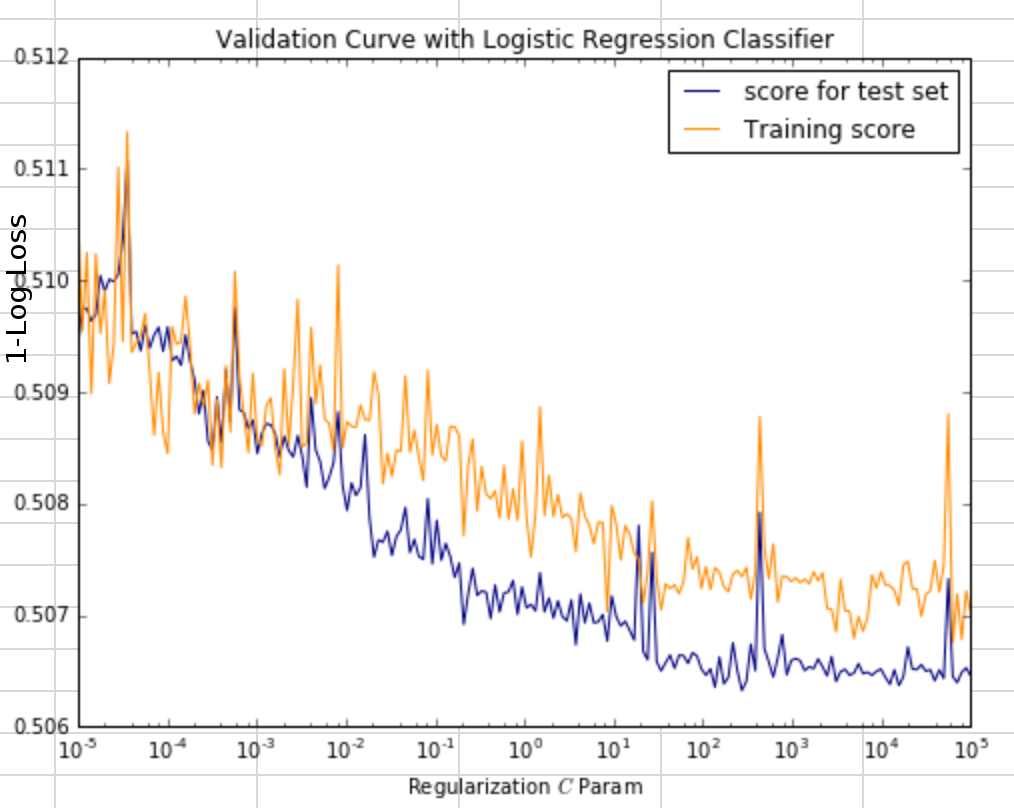
\includegraphics[width=0.7\columnwidth]{figures/regularization/figure-log_loss_error_validation_curve.png}
\caption{ Validation curve of the model's training and test sets scores using the \textit{negative log loss} and where each model is built with a different value of the $C$ regularization parameter.}
\label{fig:log_loss_regularization_validation_curve}
\end{center}
\end{figure}

For the case  showed in \cref{fig:log_loss_regularization_validation_curve}, we used all of the features from $\mathcal{T}$ and we generated multiple models $f(x,C)$ where we defined
$$C = \frac{1}{\lambda}$$

Each model was built from a specific $C$ in  $[10^{-5},10^5]$  and the model's negative log loss error was measured for the $\mathcal{T}$ and $\mathcal{T_s}$ sets separately. These errors are graphed in \cref{fig:log_loss_regularization_validation_curve} as line curves over the $C$ value.

As we can see, there is a clear tendency to have better performance across smaller values of $C$ which is equivalent to having stronger regularization of the scoring function. Note that the negative log loss will have higher values for better classifiers. Thus as a simple case and with no other manipulation of the data, we find that a regularized model helps in having a better performance across the test and train sets error.



\subsection{HyperParameters}



Note that in the model built from equation \cref{eq:logitRegularization} there are two specific parameters which must be predefined before starting the optimization procedure. Notably $\lambda$ and the $l2$ norm used to measure the size of $\theta$. These values are deemed to be \textit{hyper-parameters} of the models since they are not directly part of the theoretical construction. Also, some authors in the literature can refer to the \textit{hyper-parameters} of the model as \textit{tuning parameters}.

The hyper-parameters are the values set to configure the different possible variants in the loss function and in the model's training phase. They are values that directly affect the estimated fit $f_{\hat{\theta}}$ but are not the $\theta$ parameter themselves. They need to be instantiated before training the learner and as such, they can't be learned from the dataset.

On the other hand, in a Bayesian context the definition of hyper-parameter is different. These appear in the prior distributions of the model's parameters and should not be equated. In this case, the parameter's of $\theta$'s distribution are called the hyper-parameters.


%\textit{}


\section{Chapter Summary}\label{section-ch_machine_learning_summary}

As we know, a learner will approximate the target with $y \approx \hat{y} = h\left(\sum_{j}\theta_j x^j\right)$. The first idea led to finding the hyperplane that best separates the two classes by estimating parameter $\hat{\theta}$. Given that we now have a problem of $p$ degrees of freedom, we are left to find or fit the parameter by optimizing a certain criteria. This choice will certainly depend on the way we decide that one parameter is preferable than another. For example the choice of $0.5$ as a threshold in \cref{formula:logitThreshold} is ad-hoc and certainly one which we could try to fit in the optimization process. In the context of machine learning, loss functions give a quantitative measure of a parameter's performance. In the context of binary classification, these are also known as scoring functions.
%the criteria used to choose the best parameters

Historically, a loss function used to find the parameters would be to minimize the residual sum of squares.
We define it as is defined as $$L(z,w) = \left\Vert z-w \right\Vert^2_2$$.
This function was favored over other functions because it is more analytically tractable.

In the context of linear regression with Gaussian residuals, minimizing the residual sum of squares is equal to maximizing the likelihood probability of the target, given the input data. This results in minimizing the following sum (RSS):
%Typical of other scenarios such as linear regression, one would like

\begin{equation}\label{eq:rss}
RSS(\theta_0,..,\theta_p) = \sum_{i=1}^n {[y_i - \hat{y}_i ] }^2 \\
= \sum_{i=1}^n  {[y_i - h( \theta \cdot x_i)] }^2
\end{equation}

The equation reflects our goal to correctly match a training sample with their targets (also known as labels). Nonetheless, we are interested in having a generalized model, one which can make a \textit{good} prediction on any sample, even new ones from the true distribution of the data.
This generalization concept is lacking in the preceding equation. We'll see why it is a bad attempt to generalize the classification model constructed from the data. The idea is that because its built to fit the actual dataset which is a sample of the population. And we wouldn't expect it to perform well with any other given sample of the \textit{true} distribution for $\mathcal{T}$.
